\documentclass[a4paper, 10pt, twocolumn]{article}
% Sowohl LaTeX als auch pdfLaTeX können benutzt werden, um das Manuskript zu erstellen.

% Bitte öffnen sie diese Datei mit utf8 Zeichenkodierung!!!
\usepackage[utf8]{inputenc}         % Schriftkodierung dieser Datei
\usepackage[english]{babel}          % für deutsche Dokumente

\usepackage{nicefrac}

\usepackage{amsmath}

\usepackage{graphicx}               % optional für Grafiken
\usepackage{tabularx}               % optional für Tabellen
\usepackage{multirow}               % optional für Tabellen
\usepackage{url}                % optional für Internet Links

\usepackage[small,bf]{caption2}     % bitte für Bildunterschriften verwenden
\usepackage{parskip}
\usepackage{titlesec}
\usepackage{amsmath}                % optional für Formeln

\def\NewL{\\\noindent\hspace*{3mm}}

\titleformat{\section}{\normalfont\large\bfseries}{\thesection}{}{}
\titleformat{\subsection}{\normalfont\large\bfseries}{\thesection}{}{}
\titleformat{\paragraph}{\normalfont\bfseries}{\theparagraph}{}{}
\titlespacing{\section}{0pt}{6pt}{-1pt}
\titlespacing{\subsection}{0pt}{3pt}{-1pt}
\titlespacing{\paragraph}{0pt}{3pt}{-1pt}

\newcolumntype{Y}{>{\centering\arraybackslash}X}    %für Tabellen mit tabularx

% Definition der Seitenränder
\addtolength{\textwidth}{2.1cm}
\addtolength{\topmargin}{-2.4cm}
\addtolength{\oddsidemargin}{-1.1 cm}
\addtolength{\textheight}{4.5cm}
\setlength{\columnsep}{0.7cm}


% ADD THE FOLLOWING COUPLE LINES INTO YOUR PREAMBLE
\let\OLDthebibliography\thebibliography
\renewcommand\thebibliography[1]{
  \OLDthebibliography{#1}
  \setlength{\parskip}{0pt}
  \setlength{\itemsep}{2pt plus 0.3ex}
}

\pagestyle{empty}                   % weder Kopf- noch Fußzeile auf 1. Seite
\begin{document}
\date{}                                         % kein Datum auf 1. Seite
%\input{manuscript}





\title{\vspace{-8mm}\textbf{\large
On the Connections of High-Frequency Approximated Ambisonics and\\Wave Field Synthesis}}

% Hier die Namen und Daten der beteiligten Autoren eintragen
\author{
Frank Schultz$^1$, Gergely Firtha$^2$, Fiete Winter$^1$, Sascha Spors$^1$\\
$^1$ \emph{\small Institute of Communications Engineering, University of Rostock, 18119 Germany}\\
$^2$ \emph{\small Department of Networked Systems and Services, Budapest University of Technology and Economics, 1111 Hungary} } \maketitle
\thispagestyle{empty}           % weder Kopf- noch Fußzeile auf Folgeseiten
% Beginn des eigentlichen Manuskripts
\section*{Introduction}
\label{sec:Introduction}
\noindent\hspace*{2mm} Wave Field Synthesis (WFS) constitutes a ray-based, implicit solution of the
sound field synthesis (SFS) problem based on the Helmholtz integral equation \cite{FirthaIEEE2018}.
Explicit solutions derived in the modal domain are known for simple SFS geometries and 
fundamental virtual source types.
%
%
%
\NewL In \cite{FirthaIEEE2018} we have shown equivalence --- using a linear array
as secondary source distribution (SSD) --- of 
2\nicefrac{1}{2}-dimensional (2.5D) 
WFS and a high-frequency/far-field
approximation of the so called Spectral
Division Method (SDM) \cite[Sec. 3.7]{AhrensBook}, which constitutes the explicit SFS 
solution in Cartesian coordinates.
%
%
%
\NewL Near-field Compensated Higher Order Ambisonics (NFC-HOA)  \cite[Sec. 3.5]{AhrensBook} 
is known as the explicit
SFS solution for spherical/circular SSD geometry, for which an equivalence with WFS
is assumed as well. 
In \cite[Sec. 4.4.2]{AhrensBook} it was stated
that WFS constitutes a high-frequency approximation of 
Near-field Compensated \textit{Infinite} Order Ambisonics
by numerically evaluating the driving filter's Fourier coefficients.
%
%
%
In the present contribution further aspects and
analytic calculus are given to reinforce this claim for 2.5D SFS.


\section*{2.5D Sound Field Synthesis}
\label{sec:sfs}
\noindent\hspace*{2mm} To compare NFC-HOA and WFS for 2.5D SFS, a circular SSD is required as the modal
expansion of HOA is based on this geometry.
The  weighted superposition of monochromatic sound fields emanated by
spherical monopoles reads for $\mathrm{e}^{+\mathrm{j} \omega t}$ time convention
\begin{align}
\label{eq:SLP}
P(\mathbf{x},\omega) = \int\limits_{0}^{2\pi} D(\mathbf{x}_0,\omega) 
\frac{\mathrm{e}^{-\mathrm{j} \frac{\omega}{\mathrm{c}} |\mathbf{x}-\mathbf{x}_{0}|}}
{4\pi|\mathbf{x}-\mathbf{x}_{0}|} r_0 \, \mathrm{d}\phi_0,
\end{align}
with speed of sound $\mathrm{c}$, angular frequency $\omega$, imaginary unit $\mathrm{j}$ and SSD radius $r_0$.
Secondary sources are located at
$\mathbf{x}_0 = (r_0 \cos\phi_0,r_0 \sin\phi_0)^\mathrm{T}$.
Listening positions $r<r_0$ are denoted by
$\mathbf{x} = (r \cos\phi,r \sin\phi)^\mathrm{T}$.
%
Vector magnitude is denoted as $|\cdot|$. Inner vector product is written as
$\langle \cdot,\cdot \rangle$.
%
The inward unit normal of the SSD contour at position $\mathbf{x}_0$ is given as 
$\mathbf{\hat{n}}_0(\mathbf{x}_0) = - \frac{\mathbf{x}_0}{r_0}$.
For the discussion we use dimensionless $k r_0 = \frac{\omega}{\mathrm{c}} r_0 = \frac{2\pi}{\lambda} r_0$ and $\frac{\mathbf{x}}{\lambda}$ with the wave length $\lambda$.
%
%
%
%
\NewL Different driving filters $D(\mathbf{x}_0,\omega)$ 
realize sound fields of virtual source types $S(\mathbf{x},\omega)$,
such as e.g. i) a point source 
$S_\text{PS}(\mathbf{x},\omega) = \frac{\mathrm{e}^{-\mathrm{j} 
\frac{\omega}{\mathrm{c}} |\mathbf{x}-\mathbf{x}_\text{PS}|}}{4\pi|\mathbf{x}-\mathbf{x}_\text{PS}|} 
$
at position $\mathbf{x}_\text{PS}=(r_\text{PS} \cos\phi_\text{PS},r_\text{PS} \sin\phi_\text{PS})^\mathrm{T}$ 
with $r_\text{PS}>r_0$
and ii) a plane wave
$S_\text{PW}(\mathbf{x},\omega) = \mathrm{e}^{-\mathrm{j} \frac{\omega}{\mathrm{c}}
\langle \mathbf{\hat{k}}_\text{PW} , \mathbf{x} \rangle
}$ propagating into direction of the unit vector
$\mathbf{\hat{k}}_\text{PW} = (\cos\phi_\text{PW},\sin\phi_\text{PW})^\mathrm{T}$.
%
%
%
\newpage
\textbf{WFS Driving Filters}
%
\NewL The WFS driving filter for a virtual point source reads \cite[(2.137)]{SchultzDiss2016}
\begin{align}
D_{\text{PS,WFS}}(\mathbf{x}_0,\omega) = 
w_\text{PS}(\mathbf{x}_0) &\sqrt{8 \pi \frac{\mathrm{j \omega}}{c}} \cdot\\
\sqrt{\frac{|\mathbf{x}_0-\mathbf{x}_\text{PS}| \cdot |\mathbf{x}_\text{Ref}-\mathbf{x}_{0}|}{|\mathbf{x}_0-\mathbf{x}_\text{PS}| + |\mathbf{x}_\text{Ref}-\mathbf{x}_{0}|}}
&\langle \mathbf{\hat{k}}_\text{PS}(\mathbf{x}_0), \mathbf{\hat{n}}_0(\mathbf{x}_0)\rangle
\frac{\mathrm{e}^{- \mathrm{j} \frac{\omega}{\mathrm{c}} |\mathbf{x}_0-\mathbf{x}_\text{PS}|}}{4\pi |\mathbf{x}_0-\mathbf{x}_\text{PS}|},\nonumber
\end{align}
with the local wavenumber vector \cite{FirthaIEEE2017,FirthaIEEE2018} $\mathbf{\hat{k}}_\text{PS}(\mathbf{x}_0) = \frac{\mathbf{x}_0-\mathbf{x}_\text{PS}}{|\mathbf{x}_0-\mathbf{x}_\text{PS}|}$
and the spatial secondary source window
$w_\text{PS}(\mathbf{x}_0) = 1$ if $\langle \mathbf{\hat{k}}_\text{PS}(\mathbf{x}_0),\mathbf{\hat{n}}_0(\mathbf{x}_0)\rangle>0$
, zero otherwise.
%
The WFS driving filter for a virtual plane wave reads \cite[(2.177)]{SchultzDiss2016}
\begin{align}
\label{eq:plane_wave_WFS}
D_{\text{PW,WFS}}(\mathbf{x}_0,\omega) =
w_\text{PW}(\mathbf{x}_0) & \sqrt{8 \pi \frac{\mathrm{j \omega}}{c}}\cdot\\
\sqrt{|\mathbf{x}_\text{Ref}-\mathbf{x}_{0}|}
&\langle \mathbf{\hat{k}}_\text{PW} , \mathbf{\hat{n}}(\mathbf{x}_0) \rangle
\mathrm{e}^{- \mathrm{j} \frac{\omega}{\mathrm{c}}\langle \mathbf{\hat{k}}_\text{PW} , \mathbf{x}_0 \rangle},\nonumber
\end{align}
with the spatial secondary source window
$w_\text{PW}(\mathbf{x}_0) = 1$ if $\langle \mathbf{\hat{k}}_\text{PW} (\mathbf{x}_0),\mathbf{\hat{n}}_0(\mathbf{x}_0)\rangle>0$
, zero otherwise.
Positions of amplitude correct SFS are defineable by the specific referencing scheme linked to 
$\mathbf{x}_\text{Ref}(\mathbf{x}_0)$, cf. the referencing function discussed in 
\cite{FirthaIEEE2017}.
%
%It is worth noting that for $|\mathbf{x}_0-\mathbf{x}_\text{PS}|\gg |\mathbf{x}_\text{Ref}-\mathbf{x}_{0}|$
%and $r_\text{PS}\gg r_0$ (i.e. a virtual source very far away from the SSD resulting in a tiny wavefront curvature within the SSD)
%the point source driving filter merges to that of a plane wave
%when properly compensating the $4\pi |\mathbf{x}_0-\mathbf{x}_\text{PS}|$-amplitude and zerophase mismatch.
%
%
%

\textbf{NFC-HOA Driving Filters}
%
\NewL The NFC-HOA driving filter for a virtual point source reads \cite[Ch. 5]{AhrensBook}
\begin{align}
D_{\text{PS,HOA}}(\mathbf{x}_0,\omega) = \frac{1}{2 \pi r_0} \sum\limits_{m=-M}^{+M} \frac{h^{(2)}_{|m|}(\frac{\omega}{\mathrm{c}} r_\text{PS})}{h^{(2)}_{|m|}(\frac{\omega}{\mathrm{c}} r_0)} \mathrm{e}^{\mathrm{j} m (\phi_0 - \phi_\text{PS})},
\end{align}
using the spherical Hankel function $h_\nu^{(2)}(\cdot)$ of second kind and order $\nu$ \cite[Ch. 10]{NIST}.
%
The NFC-HOA driving function for a virtual plane wave reads \cite[Ch. 5]{AhrensBook}
\begin{align}
\label{eq:plane_wave_HOA}
D_{\text{PW,HOA}}(\mathbf{x}_0,\omega) = \frac{2 \mathrm{j}}{\frac{\omega}{\mathrm{c}} r_0} \sum\limits_{m=-M}^{+M} \frac{(-\mathrm{j})^{|m|}}{h_{|m|}^{(2)}(\frac{\omega}{\mathrm{c}} r_0)} \mathrm{e}^{\mathrm{j} m (\phi_0 - \phi_\text{PW})}.
\end{align}
%
%
%
\NewL Typically, modal order $M\leq \frac{L}{2}-1$ for a discretized SSD of even $L$ 
secondary sources is utilized to avoid spatial aliasing \cite[Sec. 4.4.1]{AhrensBook}.
%
In this paper, we are rather interested for the cases of large arguments in Hankel functions
and $M\rightarrow \infty$, i.e. a far-field/high-frequency approximation and 
infinite modal (i.e. spatial) bandwidth.
%
%
%
\section*{Amplitude Correct Synthesis}
\label{sec:ACS}
\noindent\hspace*{2mm} The origin is used as the referencing point $\mathbf{x}_\text{Ref}=\mathbf{0}$
for WFS.
This position also constitutes the expansion origin of the given NFC-HOA driving filters.
In Fig. \ref{fig:HOA_WFS_RefLine_kr20} and \ref{fig:HOA_WFS_RefLine_kr200} the
level of a virtual plane wave synthesized by NFC-HOA and WFS are depicted
for normalized wavenumber $k r_0=20$ and $k r_0=200$, respectively.
The white regions indicate amplitude correct synthesis at intended 0 dB.
For WFS, it is seen that diffraction artifacts due to the spatial window $w(\mathbf{x}_0)$
corrupt the intended sound field for
$k r_0 = 20$.
As expected, artifacts decrease for higher $k r_0$ under more valid far-field assumptions:
for $k r_0=200$ the typical positions of amplitude correct synthesis can be observed, i.e.
crescent moon like for a plane wave when using the $\mathbf{x}_\text{Ref}=\mathbf{0}$ 
referencing scheme, cf. \cite[Fig. 8]{FirthaIEEE2017}.
%
The NFC-HOA driving filter is smooth along $\mathbf{x}_0$, thus no strong diffraction
artifacts occur.
%Furthermore, since there are no far-field/high-frequency assumptions involved yet,
%the positions of amplitude correct synthesis are consistent for $k r_0=20$ and $k r_0=200$.
Fig. \ref{fig:HOA_WFS_RefLine_kr200} depicts the similarity of the positions of 
amplitude correct synthesis for NFC-HOA and WFS with chosen $\mathbf{x}_\text{Ref}=\mathbf{0}$
within the SSD.


\begin{figure}[t!]
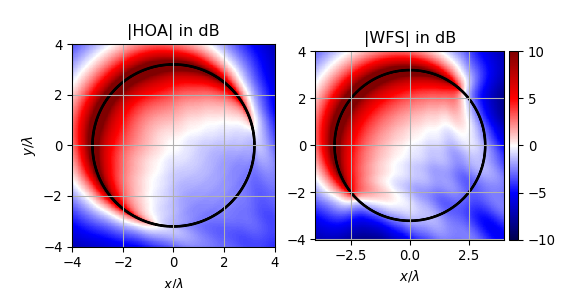
\includegraphics[width=0.5\textwidth]{HOA_WFS_RefLine_kr20.png}
\caption{Sound field's level of NFC-HOA (left) and WFS (right) synthesized virtual plane wave propagating to $\phi_\text{PW}=-\frac{\pi}{4}$ for $k r_0 = 20$.
White regions (0 dB) indicate positions of amplitude correct SFS including the origin as intended.}
\label{fig:HOA_WFS_RefLine_kr20}
\end{figure}
\begin{figure}[t!]
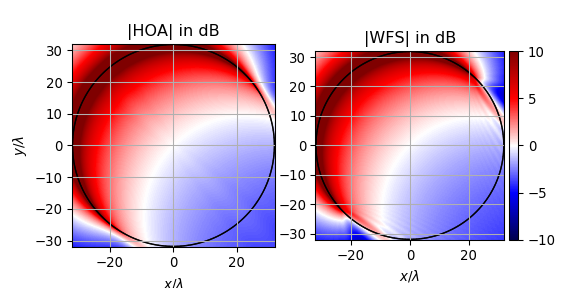
\includegraphics[width=0.5\textwidth]{HOA_WFS_RefLine_kr200.png}
\caption{Sound field's level of NFC-HOA (left) and WFS (right) synthesized virtual plane wave propagating to $\phi_\text{PW}=-\frac{\pi}{4}$ for $k r_0 = 200$.
White regions (0 dB) indicate positions of amplitude correct SFS including the origin as intended.}
\label{fig:HOA_WFS_RefLine_kr200}
\end{figure}





\section*{Stationary Phase Approximation}
\label{sec:SPA}
\noindent\hspace*{2mm} In order to evaluate the resulting sound field at a specific position, \eqref{eq:SLP}
can be treated with a stationary phase approximation (cf. \cite[App. B]{FirthaIEEE2018})
w.r.t. $\phi_0$.
%
Initially, here we evaluate the origin, our intentionally chosen reference point $\mathbf{x}_\text{Ref}=\mathbf{0}$
for WFS driving functions that constitutes the expansion center for NFC-HOA as well.
%
%
%
\NewL The SPA of \eqref{eq:SLP} using $D_{\text{PS,WFS}}(\mathbf{x}_0,\omega)$ and
$D_{\text{PW,WFS}}(\mathbf{x}_0,\omega)$ precisely results in the correct amplitude
and phase of the intended virtual sound fields $S_\text{PS}(\mathbf{x},\omega)$
and $S_\text{PW}(\mathbf{x},\omega)$, respectively, cf. \cite{Schultz2019}.
%
This is due to the single stationary secondary source $\mathbf{x}_0^* = (r_0, \phi_0^*)$ 
that is found along the line $\mathbf{x}_\text{PS} \rightarrow  \mathbf{x}_0^* \rightarrow \mathbf{0}$
for a virtual point source and along the line
$\mathbf{\hat{k}}_\text{PW} \rightarrow  \mathbf{x}_0^* \rightarrow \mathbf{0}$ (where
active secondary source selection holds as well) for a virtual plane wave, respectively.
%
%
%
%
%
%
\NewL The SPA of \eqref{eq:SLP} using $D_{\text{PS,HOA}}(\mathbf{x}_0,\omega)$ and
$D_{\text{PW,HOA}}(\mathbf{x}_0,\omega)$ in general follows the same principles, cf. \cite{Schultz2019}.
%
Since the SPA relies on far-field/high-frequency assumptions, it is meaningful to
apply a large argument approximation $h_\nu^{(2)}(z) \approx \mathrm{j}^{\nu+1} \frac{\mathrm{e}^{-\mathrm{j} z}}{z}$
within the driving functions first (which by itself is an SPA, 
the derivation can thus be performed in different ways).
For the virtual point source the large argument approximation 
$\frac{\omega}{\mathrm{c}} r_\text{PS} \rightarrow \infty$, $\frac{\omega}{\mathrm{c}} r_0 \rightarrow \infty$
yields
\begin{align}
D_{\text{PS,HOA}}(\mathbf{x}_0,\omega) \approx
\frac{1}{2 \pi r_0}
\frac
{\mathrm{e}^{-\mathrm{j} \frac{\omega}{\mathrm{c}} r_\text{PS}}}
{\mathrm{e}^{-\mathrm{j} \frac{\omega}{\mathrm{c}} r_0}}
\frac{r_0}{r_\text{PS}}
\sum\limits_{m=-M}^{+M}
\mathrm{e}^{\mathrm{j} m (\phi_0 - \phi_\text{PS})}
\end{align}
and for $M\rightarrow \infty$ the Dirichlet kernel evolves to the Dirac delta
function \cite[Sec. 1.15]{Arfken}, resulting in
\begin{align}
D_{\text{PS,HOA}}(\mathbf{x}_0,\omega) \approx
\frac{1}{r_0}
\frac
{\mathrm{e}^{-\mathrm{j} \frac{\omega}{\mathrm{c}} r_\text{PS}}}
{\mathrm{e}^{-\mathrm{j} \frac{\omega}{\mathrm{c}} r_0}}
\frac{r_0}{r_\text{PS}}
\delta(\phi_0 - \phi_\text{PS}).
\end{align}
For the virtual plane wave the large argument approximation 
$\frac{\omega}{\mathrm{c}} r_0 \rightarrow \infty$
yields
\begin{align}
D_{\text{PW,HOA}}(\mathbf{x}_0,\omega) \approx
\frac{2}{r_0} \frac{r_0}{\mathrm{e}^{-\mathrm{j} \frac{\omega}{\mathrm{c}} r_0}}
\sum\limits_{m=-M}^{+M} \, \mathrm{e}^{\mathrm{j} m (\phi_0 - \phi_\text{PWi})}
\end{align}
with the angle $\phi_\text{PWi} = \phi_\text{PW} - \pi$ for plane wave incidence rather
than propagating direction $\phi_\text{PW}$.
%
For $M\rightarrow \infty$ follows
\begin{align}
\label{eq:SPA_NFC_HOA_PW}
D_{\text{PW,HOA}}(\mathbf{x}_0,\omega) \approx
\frac{1}{r_0} \frac{4 \pi r_0}{\mathrm{e}^{-\mathrm{j} \frac{\omega}{\mathrm{c}} r_0}}
\delta(\phi_0 - \phi_\text{PWi}).
\end{align}
%
%
%
%
\NewL This case is most illustrative: By inserting driving filter 
\eqref{eq:SPA_NFC_HOA_PW} into \eqref{eq:SLP}, the sound field is generated
only by the secondary source $\mathbf{x}_0^*$ where $\phi_0 = \phi_\text{PWi}$.
The complex weight 
$4 \pi r_0 \mathrm{e}^{\mathrm{j} \frac{\omega}{\mathrm{c}} r_0}$
of this stationary secondary source compensates its amplitude decay 
towards the plane wave's unit gain amplitude in the origin and compensates its phase
shift towards the intended zero-phase of the plane wave in the origin.
%
These SPA treatments indicate that WFS and
Near-field Compensated \textit{Infinite} Order Ambisonics
 yield identical results at the origin.
%
%
%

%
%
%

\section*{Fourier Series}
\label{sec:fourier}
\noindent\hspace*{2mm} In further search of similarity or even identity of WFS and NFC-IOA not only for 
some positions or a single location, but generally for the synthesized sound field,
the equivalence of driving functions either in spatial or Fourier series domain
\begin{align}
D_{\cdot,\text{WFS}}(\mathbf{x}_0,\omega) \stackrel{?}=  D_{\cdot,\text{NFC-}\infty\text{OA}}(\mathbf{x}_0,\omega)\nonumber\\
D_{\cdot,\text{WFS}}(m,\omega) \stackrel{?}= D_{\cdot,\text{NFC-}\infty\text{OA}}(m,\omega)\nonumber
\end{align}
would be required.
While WFS is inherently given in spatial domain, NFC-HOA is analytically given 
as spatial Fourier coefficients.
Transferring both approaches to the respective corresponding domain is not 
straightforward when aiming for analytical solutions.
Here, we follow \cite[Ch. 4.4.2]{AhrensBook}, calculating a Fourier series of
the WFS driving filter.
This is performed for the virtual plane wave in detail.
The Fourier series analysis \cite[(1.84)]{NIST}
\begin{align}
D_{\cdot,\text{WFS}}(m,\omega) = 
\frac{1}{2 \pi}
\int\limits_0^{2 \pi} D_{\cdot,\text{WFS}}(\mathbf{x}_0,\omega) \cdot \mathrm{e}^{- \mathrm{j} m \phi_0 } \mathrm{d} \phi_0 
\end{align}
for the virtual plane wave \eqref{eq:plane_wave_WFS} with $\mathbf{x}_\text{Ref}=\mathbf{0}$ leads to
\cite{Schultz2019}
\begin{align}
\label{eq:WFS_FS_Conv}
&D_{\text{PW,WFS}}(m,\omega) = 
-\sqrt{8 \pi r_0 \frac{\mathrm{j \omega}}{c}} \cdot\nonumber\\
&\left[\frac{\mathrm{e}^{- \mathrm{j} m \phi_\text{PW}}}{2\,\mathrm{j}^{m-1}}
(J_{m-1}(\frac{\omega}{\mathrm{c}} r_0) - J_{m+1}(\frac{\omega}{\mathrm{c}} r_0))\right]
*_m\nonumber\\
&\left[\frac{1}{2 \pi} \frac{-\mathrm{j}}{m} (\mathrm{e}^{- \mathrm{j} m (\phi_\text{PW}+\frac{\pi}{2})}-\mathrm{e}^{- \mathrm{j} m (\phi_\text{PW}-\frac{\pi}{2}) })\right],
\end{align}
denoting the $\nu$-th order cylindrical Bessel function of first kind by $J_\nu(\cdot)$ \cite[Ch. 10]{NIST}.
%
The Fourier coefficient $D_{\text{PW,WFS}}(m,\omega)$ results from a convolution of the
sound field specific term within the first brackets (Fig. \ref{fig:kr20} top: blue) and the secondary source selection window
in the second bracket (Fig. \ref{fig:kr20} top: red). Note that the virtual source \textit{independent} term
 $J_{m-1}(\frac{\omega}{\mathrm{c}} r_0) - J_{m+1}(\frac{\omega}{\mathrm{c}} r_0) = \frac{\mathrm{d} J_{m}(\frac{\omega}{\mathrm{c}} r_0)}{\mathrm{d} (\frac{\omega}{\mathrm{c}} r_0)}$
\cite[(10.6.1)]{NIST}
is weighted by a virtual source \textit{dependent} term, here
 $\frac{\mathrm{e}^{- \mathrm{j} m \phi_\text{PW}}}{2\,\mathrm{j}^{m-1}}$ for the plane wave,
 cf. \cite{Hahn2016} for detailed treatment.
%
%
%
\begin{figure}[b!]
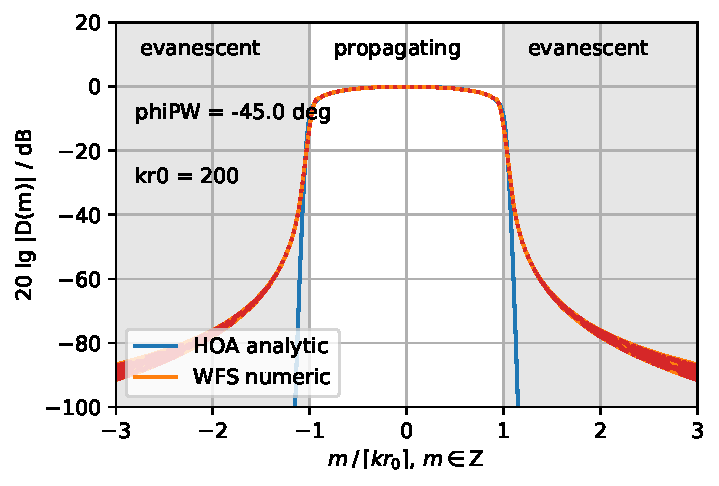
\includegraphics[width=0.5\textwidth]{nfc_hoa_vs_WFS_drivingfunctions_plot_PW_kr200_single_dB.pdf}
\caption{Level of Fourier coefficients NFC-HOA vs. WFS for virtual plane wave $\phi_\text{PW}=-\frac{\pi}{4}$, $kr_0=200$.
Note that the Fourier coefficients are continuously plotted for convenience over normalized values $m \, / \, \lceil k r_0 \rceil$.
}
\label{fig:kr200}
\end{figure}
%
%
%
\NewL The analytic complex-valued convolution in the $m$-domain is subject for further research.
%A further large-argument approximation of the involved cylindrical Bessel function was not yet successful.
Numerical convolution of the analytic terms and comparison against the 
Fourier coefficients of the NFC-HOA plane wave driving filter \eqref{eq:plane_wave_HOA}
\begin{align}
D_{\text{PW,HOA}}(m,\omega) = \frac{2 \mathrm{j}}{\frac{\omega}{\mathrm{c}} r_0} \frac{(-\mathrm{j})^{|m|}}{h_{|m|}^{(2)}(\frac{\omega}{\mathrm{c}} r_0)} \mathrm{e}^{-\mathrm{j} m \phi_\text{PW}}
\end{align}
is explored in the following.
For that we utilize the normalized spatial frequency variable $m \, / \, \lceil k r_0 \rceil$.
According to \cite[Sec. 2.2]{AhrensBook} the region
$|m \, / \, \lceil k r_0 \rceil|>1$ indicates evanescent waves, whereas
$|m \, / \, \lceil k r_0 \rceil|<1$ marks the spatial bandwidth of propagating waves.
%
%
%
%
%
%
\NewL In Fig. \ref{fig:kr200}, the level of Fourier coefficients for a virtual plane wave is depicted for NFC-HOA vs.
WFS for rather large $k r_0=200$.
In the propagating wave region the levels highly match, whereas WFS exhibits
more energy in the evanescent wave region.
This is again due to the discontinuous secondary source selection window 
compared to the smoother driving control in NFC-HOA, cf. \cite[p.95]{SchultzDiss2016}.
This artifact only completely vanishes when $k r_0\rightarrow\infty$.
This in turn requires infinite spatial bandwidth $M\rightarrow\infty$ for NFC-HOA. 
%
%
%
\NewL A more detailed picture on the Fourier coefficients is presented in Fig. 
\ref{fig:kr20} using rather low $k r_0=20$ for clarity.
The top row shows the real and imaginary part of the WFS-specific functions
\eqref{eq:WFS_FS_Conv} involved in the convolution.
The middle and bottom rows compare NFC-HOA against WFS w.r.t. real and imaginary part,
magnitude and level of Fourier coefficients.
These plots indicate good similarity, but no equivalence of the two approaches.
Here, for WFS even higher energy for evanescent waves can be observed compared to Fig. 
\ref{fig:kr200} with $k r_0=200$.


\begin{figure*}
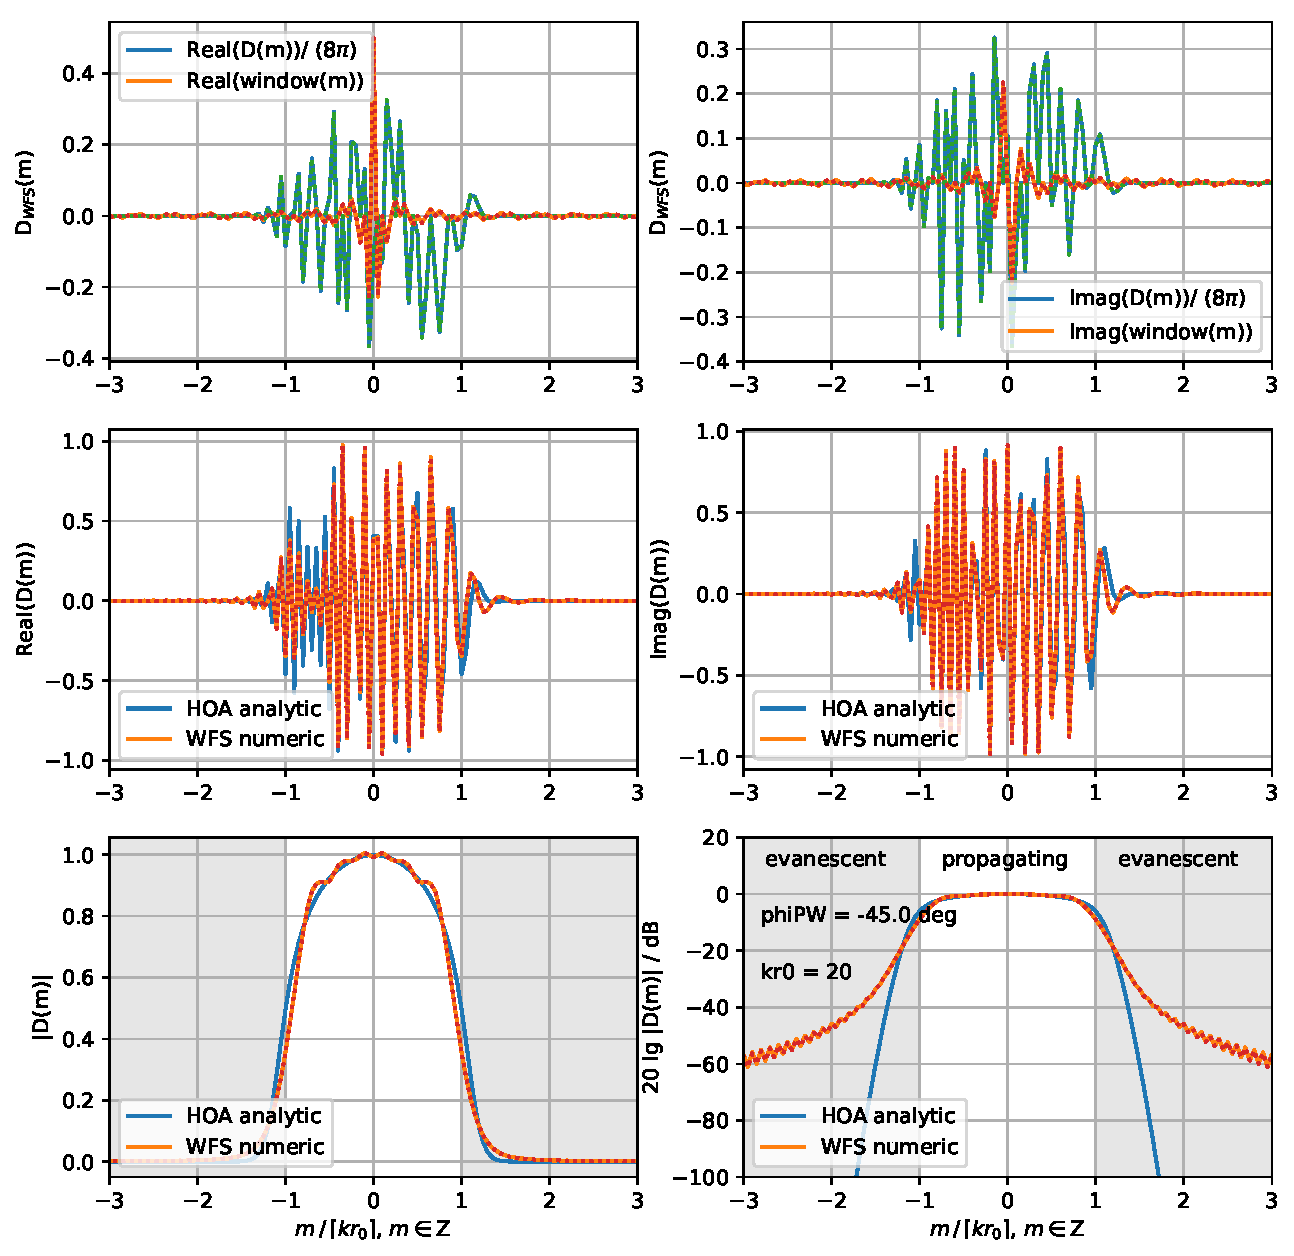
\includegraphics[width=\textwidth]{nfc_hoa_vs_WFS_drivingfunctions_plot_PW_kr20.pdf}
\caption{Fourier coefficients of plane wave driving filter for NFC-HOA vs. WFS, $kr_0=20$, $\phi_\text{PW}=-\frac{\pi}{4}$.
\textbf{Top row}: WFS split into real (left) and imaginary (right) part, sound field specific part (blue) $*_m$ spatial secondary source selection window (red).
\textbf{Middle row}: comparison of Fourier coefficients, real (left) and imaginary (right), NFC-HOA (blue) vs. WFS (red).
\textbf{Bottom row}: magnitude (left) and level (right) of middle row scenario.
Note that the Fourier coefficients are continuously plotted for convenience over normalized values $m \, / \, \lceil k r_0 \rceil$.
Plots created with \cite[\texttt{nfc\_hoa\_vs\_WFS\_drivingfunctions\_PW.py}]{Schultz2019}.}
\label{fig:kr20}
\end{figure*}








\section*{Conclusion}
\label{sec:Conclusion}
\noindent\hspace*{2mm} Although a strict proof is not yet available, the present treatment supports
the initial claim, that Near-field Compensated \textit{Infinite} Order Ambisonics
and Wave Field Synthesis with inherently infinite spatial bandwidth  
behave identically if i) referencing and expansion to the origin
is performed and ii) high-frequency/far-field assumptions are fulfilled.
The normalized wave number $k r_0 \rightarrow \infty$ then requires modal order $M\rightarrow \infty$
and vice versa.

\section*{Acknowledgement}
\noindent\hspace*{2mm} We thank Nara Hahn for helpful comments.

\small
\begin{thebibliography}{99}
\bibitem{FirthaIEEE2018}
G. Firtha et al. (2018): "On the General Relation of Wave Field Synthesis 
and Spectral Division Method for Linear Arrays." \textit{IEEE TASLP} \textbf{26}(12):2393-2403.
%\url{https://doi.org/10.1109/TASLP.2018.2865091}


\bibitem{AhrensBook}
J. Ahrens (2012): \textit{Analytic Methods of Sound Field Synthesis}. Springer.
%\url{https://doi.org/10.1007/978-3-642-25743-8}


\bibitem{SchultzDiss2016}
F. Schultz (2016): \textit{Sound Field Synthesis for Line Source Array Applications 
in Large-Scale Sound Reinforcement}. doctoral thesis, University of Rostock.
%\url{https://doi.org/10.18453/rosdok_id00001765}


\bibitem{FirthaIEEE2017}
G. Firtha et al. (2017): "Improved Referencing Schemes for 2.5D Wave Field
Synthesis Driving Functions." \textit{IEEE TASLP} \textbf{25}(5):1117-1127.
%\url{https://doi.org/10.1109/TASLP.2017.2689245}


\bibitem{NIST}
F.W.J. Olver et al. (2019, version 1.0.22): NIST Digital Library of Mathematical Functions.
%\url{https://dlmf.nist.gov/}


\bibitem{Arfken}
G.B. Arfken et al. (2005): \textit{Mathematical Methods for Physicists}. Elsevier, 6th ed.


\bibitem{Schultz2019}
\url{https://github.com/spatialaudio/sfs-with-local-wavenumber-vector-concept}



\bibitem{Hahn2016}
N. Hahn et al. (2016): "Local Wave Field Synthesis by Spatial Band-limitation 
in the Circular/Spherical Harmonics Domain." \textit{Proc. 140th Audio Eng. Soc. Conv.}
Paris.
%\url{http://www.aes.org/e-lib/browse.cfm?elib=18294}



















\end{thebibliography}





























\end{document}


% DAGA2019/338
% On the Connections of High-Frequency Approximated Ambisonics and Wave Field Synthesis
% Frank Schultz, Gergely Firtha, Fiete Winter und Sascha Spors
% Universität Rostock, Institut für Nachrichtentechnik
% Budapest University of Technology frank.schultz@uni-rostock.de
% From numeric 2.5D sound field synthesis (SFS) it is known that the 
% spatially-fullband technique Wave Field Synthesis (WFS) constitutes a 
% high-frequency approximation of Near-Field Compensated Infinite Order 
% Ambisonics. Recently, the authors have analytically shown equivalence of 2.5D 
% WFS and a high-frequency/far-field approximation of the Spectral Division Method
%  (SDM) using linear arrays. SDM constitutes the explicit SFS solution in cartesian
%   coordi- nates. This contribution therefore aims at showing equivalence of the 
%   explicit solution in circular/spherical coordinates, namely Ambisonics, and 
%   the WFS. For that the recently introduced local wavenumber vector concept 
%   is utilised, which essentially links SFS approaches to geometric acoustics.